%%%%%%%%%%%%  Generated using docx2latex.pythonanywhere.com  %%%%%%%%%%%%%%
\documentclass[a4paper,12pt,oneside]{report}
% Other options in place of 'report' are 1)article 2)book 3)letter
% Other options in place of 'a4paper' are 1)a5paper 2)b5paper 3)letterpaper 4)legalpaper 5)executivepaper
%%%%%%%%%%%%  Include Packages  %%%%%%%%%%%%%%
\usepackage{amsmath}%,amssymb,amsthm}
% \usepackage{latexsym}
% \usepackage{amsfonts}
\usepackage{graphicx}
\usepackage{txfonts}
% \usepackage{wasysym}
\usepackage{enumitem}
% \usepackage{adjustbox}
% \usepackage{ragged2e}
% \usepackage{tabularx}
% \usepackage{changepage}
% \usepackage{setspace}
% \usepackage{hhline}
% \usepackage{multicol}
% \usepackage{float}
% \usepackage{multirow}
% \usepackage{makecell}
\usepackage{fancyhdr}
% \usepackage[toc,page]{appendix}
% \usepackage[utf8]{inputenc}
% \usepackage[T1]{fontenc}
\usepackage{hyperref}
% \usepackage{isomath}
% \usepackage{fixmath}
% \usepackage{tikz}
% \usepackage{textcomp}
% \usepackage{epstopdf} %converting to PDF
% \usepackage{upgreek}
% \usetikzlibrary{shapes,shadows,arrows,calc}
% \usetikzlibrary{decorations.pathreplacing,decorations.markings,shapes.geometric}
% \usepackage[toc,page]{appendix}
% %general:
%Box and color definitions:
%--------------------------
\newenvironment{ColorBoxedminipage}
{\begin{minipage}} {\end{minipage}}
%{\begin{Sbox}\begin{minipage}}
%{\end{minipage}\end{Sbox}\fcolorbox{Blue}{White}{\TheSbox}}

\newcommand{\sheading}[1]{
  \large\bf
  \textcolor{NavyBlue}{\begin{Bcenter}#1\end{Bcenter}}}

\setlength{\fboxsep}{0.35cm} \setlength{\fboxrule}{4pt}

\definecolor{LightBlue}{rgb}{0.8,0.85,1}
\definecolor{LightGreen}{rgb}{0,1,.85}
\definecolor{BrickRed}{named}{BrickRed}
\definecolor{Black}{named}{Black}
\definecolor{PineGreen}{named}{PineGreen}
\definecolor{Green}{named}{Green}
\definecolor{Red}{named}{Red}
\definecolor{NavyBlue}{named}{NavyBlue}
\definecolor{WildStrawberry}{named}{WildStrawberry}
\definecolor{White}{named}{White}
\definecolor{CadetBlue}{named}{CadetBlue}
\definecolor{Blue}{named}{Blue}

%General definitions:
%-------------------
%\newcommand{\PlotPath}{e:/thesa/latex/thesa_plots/}
\newcommand{\PlotPath}{y:/thesa_plots/}
\newcommand{\inp}[2]{\left<{{#1},{#2}}\right>} %inner product
\newcommand{\etal}{{\em {et al.}}}
\newcommand{\B}[1]{\mathbf{#1}}
\newcommand{\df}{\triangleq}
\newcommand{\W}{\omega}
\newcommand{\norm}[1]{\left\Vert#1\right\Vert}
\newcommand{\abs}[1]{\left\vert#1\right\vert}
\newcommand{\RE}{\operatorname{Re}}
\newcommand{\IM}{\operatorname{Im}}
\newcommand{\sgma}[3]{\sum\limits_{{#1}={#2}}^{#3}}
\newcommand{\Brk}[1]{\left(#1\right)} %Put argument in brackets
\newcommand{\E}[1]{E\left\{#1\right\}} %Expectation
\newcommand{\Var}[1]{Var\left\{#1\right\}} %Variance
\newcommand{\Cov}[1]{Cov\left\{#1\right\}} %Covariance
\newcommand{\Brace}[1]{\left\{{#1}\right\}} %Braces
\newcommand{\Brack}[1]{\left({#1}\right)} %Brackets
\newcommand{\sBrack}[1]{\left[{#1}\right]} %square Brackets
\newcommand{\Mtr}[2] %short notation for 2x1 Matrix.
{\begin{bmatrix}
  #1 \\
  #2
\end{bmatrix}}
\newcommand{\cMtr}[2] %short notation for 2x1 Matrix with curves.
{\left(
\begin{array}{c}
    {#1} \\
    {#2} \\
\end{array}
\right)}
\newcommand{\Mtrs}[2] %short notation for 2x1 Matrix star (adjoint)
{\begin{bmatrix}
  #1 &
  #2
\end{bmatrix}}
\newcommand{\Mtrt}[3] %short notation for 3x1 Matrix.
{\begin{bmatrix}
  #1 \\
  #2 \\
  #3
\end{bmatrix}}

\newcommand{\Cases}[4]{
\left\{
\begin{tabular}{lcl}
    $#1$ & $=$ & $#2$\\
    $#3$     & $=$ & $#4$
\end{tabular}
\right. }

\newcommand{\und}{\underline} %How lazy can I get?
\newcommand{\ovr}{\overline}
\newcommand{\conj}[1]{{#1}^\ast} %Conjugation

\newcommand{\ls}[2]{\Brk{\conj{#1} {#1}}^{-1}\conj{#1}{#2}} %LS
\newcommand{\wls}[3]{\Brk{\conj{#1}{#3}{#1}}^{-1}\conj{#1}{#3}{#2}} %weighted LS

\newcommand{\iter}[1]{^{({#1})}}
\newcommand{\ut}{\und{\theta}} %underline theta
\newcommand{\us}{\und{s}} %underline s.
\newcommand{\usk}[1]{\und{s}^{(#1)}} %underline s at k-th iteration
\newcommand{\ust}[1]{\und{s}({#1})} %underline s at time t
\newcommand{\ti}[1]{\und{\theta}^{(#1)}} %theta^(i)
\newcommand{\tli}[1]{\und{\theta}{(#1)}} %theta low i: theta_i (for time indexing)
\newcommand{\htli}[1]{\hat{\und{\theta}}{(#1)}} %theta low i: theta_i (for time indexing)



%identity matrices:
\newcommand{\It}{I_2}
\newcommand{\Io}{I_1}
\newcommand{\uz}{\und{0}} %underline Zero
\newcommand{\uo}{\und{1}} %underline One


%Power spectrum shortcuts:
\newcommand{\nw}[1]{({#1},\W)}
\newcommand{\Ps}{\Phi_{ss}(\W)}
\newcommand{\Psk}[1]{\Phi_{ss}({#1},\W)}
\newcommand{\Pn}{\Phi_{nn}(\W)}
\newcommand{\uPn}{\und{\Phi}_{nn}(\W)} %underline Pnn
\newcommand{\Poo}{\Phi_{z_1z_1}(\W)} %P one one
\newcommand{\hPoo}{\hat{\Phi}_{z_1z_1}(\W)} %hat P one one
\newcommand{\uPoo}{\und{\Phi}_{z_1z_1}(\W)} %underline P one one
\newcommand{\uhPoo}{\hat{\und{\Phi}}_{z_1z_1}(\W)} %underline hat P one one
\newcommand{\Pook}[1]{\hat{\Phi}_{z_1z_1}\nw{#1}} %the argument is the frame index.
\newcommand{\Pot}{\Phi_{z_1z_2}(\W)} %P one two
\newcommand{\Pto}{\Phi_{z_2z_1}(\W)} %P two one
\newcommand{\Ptt}{\Phi_{z_2z_2}(\W)} %P two two
\newcommand{\Pom}{\Phi_{z_1z_m}(\W)} %P one m
\newcommand{\Pij}{\Phi_{z_iz_j}(\W)} %P i j
\newcommand{\Pii}{\Phi_{z_iz_i}(\W)} %P i i
\newcommand{\Pjj}{\Phi_{z_jz_j}(\W)} %P j j
\newcommand{\hPij}{\hat{\Phi}_{z_iz_j}(\W)} %hat P i j
\newcommand{\hPom}{\hat{\Phi}_{z_1z_m}(\W)} %P one m
\newcommand{\uPom}{\und{\Phi}_{z_1z_m}(\W)} %underline P one m
\newcommand{\uhPom}{\und{\hat{\Phi}}_{z_1z_m}(\W)} %underline hat P one m
\newcommand{\Pmo}{\Phi_{z_mz_1}(\W)} %P m one
\newcommand{\hPmo}{\hat{\Phi}_{z_mz_1}(\W)} % hat P m one
\newcommand{\uPmo}{\und{\Phi}_{z_mz_1}(\W)} %underline P m one
\newcommand{\uhPmo}{\und{\hat{\Phi}}_{z_mz_1}(\W)} %underline hat P m one
\newcommand{\Pmok}[1]{\hat{\Phi}_{z_mz_1}\nw{#1}} %the argument is the frame index.
\newcommand{\Pomk}[1]{\hat{\Phi}_{z_1z_m}\nw{#1}} %the argument is the frame index.
\newcommand{\Pmmk}[1]{\hat{\Phi}_{z_mz_m}\nw{#1}} %the argument is the frame index.
\newcommand{\Pmm}{\Phi_{z_mz_m}(\W)} %P m m
\newcommand{\hPmm}{\hat{\Phi}_{z_mz_m}(\W)} %hat P m m
\newcommand{\uPmm}{\und{\Phi}_{z_mz_m}(\W)} %underline P m m
\newcommand{\uhPmm}{\und{\hat{\Phi}}_{z_mz_m}(\W)} %underline hat P m m
\newcommand{\Pz} %Pz matrix
{\begin{bmatrix}
  \Poo & \Pom\\
  \Pmo & \Pmm
\end{bmatrix}}
%decorrelation matrix stuff
\newcommand{\uow}{u_1(\W)}
\newcommand{\utw}{u_2(\W)}
\newcommand{\utwn}{\conj{u}_2(\W)}


%\newcommand{\Pu}{{\Phi}_{\check{n}}(\W)}
\newcommand{\biasOne}{b_1} %will be used for the PSD and the correlation.
\newcommand{\Pbo}{{\Phi}_{\biasOne}(\W)} %P bias one
\newcommand{\Pbok}[1]{{\Phi}_{\biasOne}^{(#1)}(\W)} %P bias one, at the k-th iteration
\newcommand{\hPbo}{{\hat{\Phi}}_{\biasOne}(\W)} %hat P bias one
\newcommand{\hPbot}[1]{{\hat{\Phi}}_{\biasOne}({#1},\W)} %hat P bias one at the t-th time instance
\newcommand{\biasm}{b_m} %The seond bias. will be used for the PSD
\newcommand{\Pbm}{{\Phi}_{\biasm}(\W)} %P bias m
\newcommand{\hPbm}{\hat{\Phi}_{\biasm}(\W)} %P bias m


%Signals Fourier transforms:
\newcommand{\N}{N(\W)} %N
\newcommand{\Sig}{S(\W)} %S
\newcommand{\Zo}{Z_1(\omega)} %Z one
\newcommand{\Zt}{Z_2(\omega)} %Z two

%Transfer functions:
\newcommand{\Ao}{{A_1(\omega)}}
\newcommand{\At}{{A_m(\omega)}}
\newcommand{\Am}{{A_m(\omega)}}
\newcommand{\Bo}{{B_1(\omega)}}
\newcommand{\Bt}{{B_m(\omega)}}
\newcommand{\Bm}{{B_m(\omega)}}
\newcommand{\Aon}{\conj{A_1}(\omega)}
\newcommand{\Amn}{\conj{A_m}(\omega)}
\newcommand{\Bon}{\conj{B_1}(\omega)}
\newcommand{\Bmn}{\conj{B_m}(\omega)}
\newcommand{\Hm}{{\mathcal{H}_m(\omega)}}
\newcommand{\Hmk}[1]{{\mathcal{H}_m^{(#1)}(\omega)}}
\newcommand{\hHm}{{\hat{\mathcal{H}}_m(\W)}} %hat Hm
\newcommand{\hHmt}[1]{{\hat{\mathcal{H}}_m({#1},\W)}} %hat Hm at the t-th time instance
\newcommand{\Gm}{{\mathcal{G}_m(\W)}}
\newcommand{\Gmn}{\conj{\mathcal{G}}_m(\W)} %conj Gm
\newcommand{\Gmnk}[1]{\conj{\mathcal{G}_m^{(#1)}}(\W)} %conj Gm at the k-th iteration
\newcommand{\hGmnt}[1]{\conj{\hat{\mathcal{G}}}_m({#1},\W)} %hat conj Gm at the t-th time instance.
\newcommand{\Ar}{\frac{\Am}{\Ao}} % Am/A1 ratio
\newcommand{\Br}{\frac{\Bm}{\Bo}} % Bm/B1 ratio

%Impulse response shortcuts:
\newcommand{\hm}{h_m}
\newcommand{\hhm}{\hat{h}_m} %hat hm
\newcommand{\uhm}{\und{h}_m} %underlined hm
\newcommand{\uhhm}{\und{\hat{h}}_m} %underlined hm
\newcommand{\ao}{a_1} %a one
\newcommand{\at}{a_2} %a two
\newcommand{\am}{a_m} %a m
\newcommand{\bo}{b_1} %b one
%\newcommand{\bt}{b_2} %b two
%\newcommand{\bm}{b_m} %b m


%Special notations for transfer function ratios (related to decorrelation):
\newcommand{\ko}{k_1(\omega)} %k one
\newcommand{\ktw}{k_2(\omega)} %k two
\newcommand{\kt}{k_3(\omega)} %k three
\newcommand{\kon}{\overline{\ko}} %k one negate
\newcommand{\ktwn}{\overline{\ktw}} %k two negate
\newcommand{\ktn}{\overline{\kt}} %k three negate

%Correlation shortcuts:
\newcommand{\Roo}{R_{z_1z_1}} %R one one
\newcommand{\Rmo}{R_{z_mz_1}} %R m one
\newcommand{\Rhoo}{\hat{R}_{z_1z_1}} %R hat one one
\newcommand{\Rhook}[1]{\Rhoo^{(#1)}} %R hat one one at k'th (n'th) frame
\newcommand{\uRhoo}{{\underline \Rhoo}} %underlined R hat one one
\newcommand{\uRhook}[1]{\underline {\Rhoo^{(#1)}}} %underlined R hat one one at k'th (n'th) frame
%\newcommand{\Rto}{R_{z_2z_1}} %R two one
\newcommand{\Rhmo}{\hat{R}_{z_mz_1}} %R hat m one
\newcommand{\Rhmok}[1]{\Rhmo^{(#1)}} %R hat m one at k'th frame
\newcommand{\uRhmo}{{\und{\hat{R}}_{z_mz_1}}} %underlined R hat m one
\newcommand{\uRhmok}[1]{\und{\hat{R}}_{z_mz_1}^{(#1)}} %underlined R hat m one at k'th frame
\newcommand{\Rhu}{\hat{R}_{\check{n}}} %the noise bias vector
\newcommand{\Too}{\hat{\B{T}}_{z_1z_1}} %T one one (Toeplitz matrix for z1 z1)
\newcommand{\Took}[1]{\Too^{(#1)}} %T one one (Toeplitz matrix for z1 z1) at k'th frame
\newcommand{\Rbo}{R_{\biasOne}} %R bias one
\newcommand{\uRbo}{\und{R}_{\biasOne}} %underlined R noise one
\newcommand{\uhRbo}{\hat{\und{R}}_{\biasOne}} %underlined hat R noise one

\newenvironment{alg}[5]
{
\begin{figure}[htbp]
\begin{center}
\fbox{
  \begin{ColorBoxedminipage}{13cm}
%    \leftline{\color{Black}\bf {#1}}
    {#4}
   \end{ColorBoxedminipage}
   }
\end{center}
  \bcaptionff{#1}{#2}{}{#3}
  \label{#5}
\end{figure}
}{}

%general:
%Box and color definitions:
%--------------------------
\newenvironment{ColorBoxedminipage}
{\begin{minipage}} {\end{minipage}}
%{\begin{Sbox}\begin{minipage}}
%{\end{minipage}\end{Sbox}\fcolorbox{Blue}{White}{\TheSbox}}

%General definitions:
%-------------------
\newcommand{\etal}{{\em {et al.}}}
\newcommand{\B}[1]{\mathbf{#1}}
\newcommand{\df}{\triangleq}
\newcommand{\norm}[1]{\left\Vert#1\right\Vert}
\newcommand{\abs}[1]{\left\vert#1\right\vert}
\newcommand{\RE}{\operatorname{Re}}
\newcommand{\IM}{\operatorname{Im}}
\newcommand{\sgma}[3]{\sum\limits_{{#1}={#2}}^{#3}}
\newcommand{\Brace}[1]{\left\{{#1}\right\}} %Braces
\newcommand{\Brack}[1]{\left({#1}\right)} %Brackets
\newcommand{\sBrack}[1]{\left[{#1}\right]} %square Brackets

%\newcommand{\ip}[2]{{\langle{#1},{#2}\rangle}} %inner-product
\newcommand{\ipLW}[3]{{\langle{#1},{#2}\rangle}_{{#3}}} %weighted inner-product

\newcommand{\Tr}[1]{Tr\Brack{#1}}
\newcommand{\Mtr}[2] %short notation for 2x1 Matrix.
{\begin{bmatrix}
  #1 \\
  #2
\end{bmatrix}}
\newcommand{\cMtr}[2] %short notation for 2x1 Matrix with curves.
{\left(
\begin{array}{c}
    {#1} \\
    {#2} \\
\end{array}
\right)}
\newcommand{\Mtrs}[2] %short notation for 2x1 Matrix star (adjoint)
{\begin{bmatrix}
  #1 &
  #2
\end{bmatrix}}
\newcommand{\Mtrt}[3] %short notation for 3x1 Matrix.
{\begin{bmatrix}
  #1 \\
  #2 \\
  #3
\end{bmatrix}}

\newcommand{\Cases}[4]{
\left\{
\begin{tabular}{lcl}
    $#1$ & $=$ & $#2$\\
    $#3$     & $=$ & $#4$
\end{tabular}
\right. }

\newcommand{\und}{\underline} %How lazy can I get?
\newcommand{\ovr}{\overline}
\newcommand{\conj}[1]{{#1}^\ast} %Conjugation


\newcommand{\er}[1]{{(\ref{#1})}} %equation reference

\newtheorem{Lemma}{Lemma}{}
\newtheorem{Prop}{Proposition}{}
\newtheorem{theorem}{Theorem}{}


\newenvironment{alg}[5]
{
\begin{figure}[htbp]
\begin{center}
\fbox{
  \begin{ColorBoxedminipage}{13cm}
%    \leftline{\color{Black}\bf {#1}}
    {#4}
   \end{ColorBoxedminipage}
   }
\end{center}
  \bcaptionff{#1}{#2}{}{#3}
  \label{#5}
\end{figure}
}{}

%Just body, caption and label.
\newenvironment{algo}[3]
{
\begin{figure}[htbp]
\begin{center}
\fbox{
  \begin{ColorBoxedminipage}{7.5cm}
%    \leftline{\color{Black}\bf {#1}}
    {#1}
   \end{ColorBoxedminipage}
   }
\end{center}
  \caption{#2}
  \label{#3}
\end{figure}
}{}

\newenvironment{BOX}[1]
{
\begin{center}
\fbox{
  \begin{ColorBoxedminipage}{16cm}
%    \leftline{\color{Black}\bf {#1}}
    {#1}
   \end{ColorBoxedminipage}
   }
\end{center}
}{}

\newcommand\vecnot[1]{\boldsymbol{#1}}
\newcommand\optvecnot[1]{\vecnot{#1}_{opt}}

\usepackage{amsmath}
\DeclareMathOperator*{\argmax}{arg\,max}
\DeclareMathOperator*{\argmin}{arg\,min}
%%%%%%%%%%%%  Define Colors For Hyperlinks  %%%%%%%%%%%%%%
\hypersetup{
colorlinks=true,
linkcolor=blue,
filecolor=magenta,
urlcolor=cyan,
}
\urlstyle{same}
%%%%%%%%%%%%  Set Depths for Sections  %%%%%%%%%%%%%%
% 1) Section
% 1.1) SubSection
% 1.1.1) SubSubSection
% 1.1.1.1) Paragraph
% 1.1.1.1.1) Subparagraph
\setcounter{tocdepth}{5}
\setcounter{secnumdepth}{5}
%%%%%%%%%%%%  Set Page Margins  %%%%%%%%%%%%%%
\usepackage[a4paper,bindingoffset=0.2in,headsep=0.5cm,left=1.25in,right=1.25in,bottom=2cm,top=2cm,headheight=2cm]{geometry}
\everymath{\displaystyle}
%%%%%%%%%%%%  Set Depths for Nested Lists created by \begin{enumerate}  %%%%%%%%%%%%%%
\setlistdepth{9}
\newlist{myEnumerate}{enumerate}{9}
\setlist[myEnumerate,1]{label=\arabic*)}
\setlist[myEnumerate,2]{label=\alph*)}
\setlist[myEnumerate,3]{label=(\roman*)}
\setlist[myEnumerate,4]{label=(\arabic*)}
\setlist[myEnumerate,5]{label=(\Alph*)}
\setlist[myEnumerate,6]{label=(\Roman*)}
\setlist[myEnumerate,7]{label=\arabic*}
\setlist[myEnumerate,8]{label=\alph*}
\setlist[myEnumerate,9]{label=\roman*}
\renewlist{itemize}{itemize}{9}
\setlist[itemize]{label=$\cdot$}
\setlist[itemize,1]{label=\textbullet}
\setlist[itemize,2]{label=$\circ$}
\setlist[itemize,3]{label=$\ast$}
\setlist[itemize,4]{label=$\dagger$}
\setlist[itemize,5]{label=$\triangleright$}
\setlist[itemize,6]{label=$\bigstar$}
\setlist[itemize,7]{label=$\blacklozenge$}
\setlist[itemize,8]{label=$\prime$} 
%%%%%%%%%%%%  Header here  %%%%%%%%%%%%%%
\pagestyle{fancy}
\fancyhf{}
%%%%%%%%%%%%  Footer here  %%%%%%%%%%%%%%
%%%%%%%%%%%%  Print Page Numbers  %%%%%%%%%%%%%%
\rfoot{\thepage}
%%%%%%%%%%%%  This sets linespacing (verticle gap between Lines) Default=1 %%%%%%%%%%%%%%
\setstretch{1.15}
%%%%%%%%%%%%  Document Code starts here %%%%%%%%%%%%%%
\author{
Yehezkel Karo Itay\\[1cm]{Supervisor: Prof. Cohen Israel}\\{External supervisor: Dr. Dvorkind Tsvi}
}
\title{Spatial IIR processing – Thesis proposal}
\begin{document}
\maketitle
\sloppy 
 \par
\noindent 
\section*{Abstract}
Uniform linear array (ULA) processing in the spatial domain is similar to time domain finite-impulse-response (FIR) filtering (e.g. \cite{van1988beamforming}).
The similarity arises because temporal FIR's input is composed of equally time-spaced samples and the ULA's input is obtained from equally spatially-spaced samples of the impinging wavefront.
Both temporal FIR and ULA filtering assign weights to each sample in order to achieve a desired temporal/spatial response.
From time domain filter design theory, it is well known that infinite impulse response (IIR) filters attain certain advantages over FIR filtering.
The described method is illustrated in Fig. \ref{fig:SpatialIIR_SubArrays}.
\begin{figure}[!h]
\begin{center}
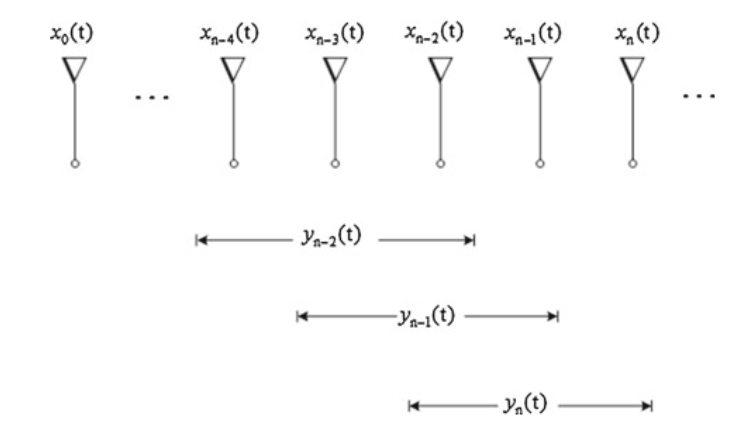
\includegraphics[width=0.7\textwidth]{./Media/SpatialIIR_SubArrays.PNG}
\caption{The sub-array solution for the spatial auto-regressive part of the filter, as implemented in \cite{wen2013array}.}
\label{fig:SpatialIIR_SubArrays}
\end{center}
\end{figure}
A natural question to consider is ``what is the array structure in spatial domain which is analogous to IIR filtering in the time domain?''.
The motivation for finding an IIR equivalent in the spatial domain is obvious:
\begin{itemize}
\item
{
Increased degrees of freedom over conventional array processing to control the array response.
}
\item
{
Substantially lower number of taps (smaller number of array elements and reduced array aperture) is required for obtaining a desired response in comparison to an FIR based design. This, naturally, results in cost-efficient array.
}
\end{itemize}
In his PhD thesis \cite{wen2013array}, Wen presented the same question. In his work two approaches were suggested for achieving ``spatial-IIR'' filtering.
First was to use shifted-sub-arrays, in order to approximate the auto-regressive part of the filter.
In practice, this approximation is equivalent to a truncated response of the IIR filter thus obtaining only an FIR implementation.
The second approach in \cite{wen2013array}, was to estimate the DOA of the impinging signal and approximate the auto-regressive part of the filter by temporal processing.
The latter approach is speculated to be very sensitive to DOA estimation errors; and it is not clear how one may extend this approach to multiple speakers scenario.
Additional works \cite{Madanayake2008ABeamformer,Madanayake2009SystolicWDFs,Madanayake2008AFilters,Bruton2003Three-dimensionalBanks,Ward1986ABeamforming,Joshi2012SynthesisApplications} consider a different approach of 2-D spatio-temporal filtering. In particular, the wavefront is viewed as a two dimensional signal, and the processing is done by performing IIR filtering in the time domain, but only FIR filtering (using a finite number of sensors) is performed in the spatial domain.
As can be seen in \cite{Bruton2003Three-dimensionalBanks}, the obtained 2-D filter is not ideal, causing imperfections in the overall spatial response.
\\
In this work we propose spatial-IIR filtering. As time-domain filter design relies on feeding back the filter's input with a combination of its taps, our approach relies on spatial feedback of received array signals back to the transmitter.
In the context of acoustic signal processing, a cooperative speaker will hold an electronic or acoustic transponder. 
Thus, the received signals at a microphone array will consist of the direct speech signal of the speaker, and a feedback signal which was recorded by the array at a previous time epoch (see Fig. \ref{fig:SignalModel}). 
Naturally, this suggested approach requires a cooperative speaker/source but, as will be explained, spatial-only-IIR filtering will be achieved by this scheme.
Comparing to \cite{wen2013array}, our method solves the main issues of both suggested approaches, achieving spatial IIR processing of multiple speaker scenarios.
\section*{Suggested schematic}
\begin{figure}[!ht]
\begin{center}
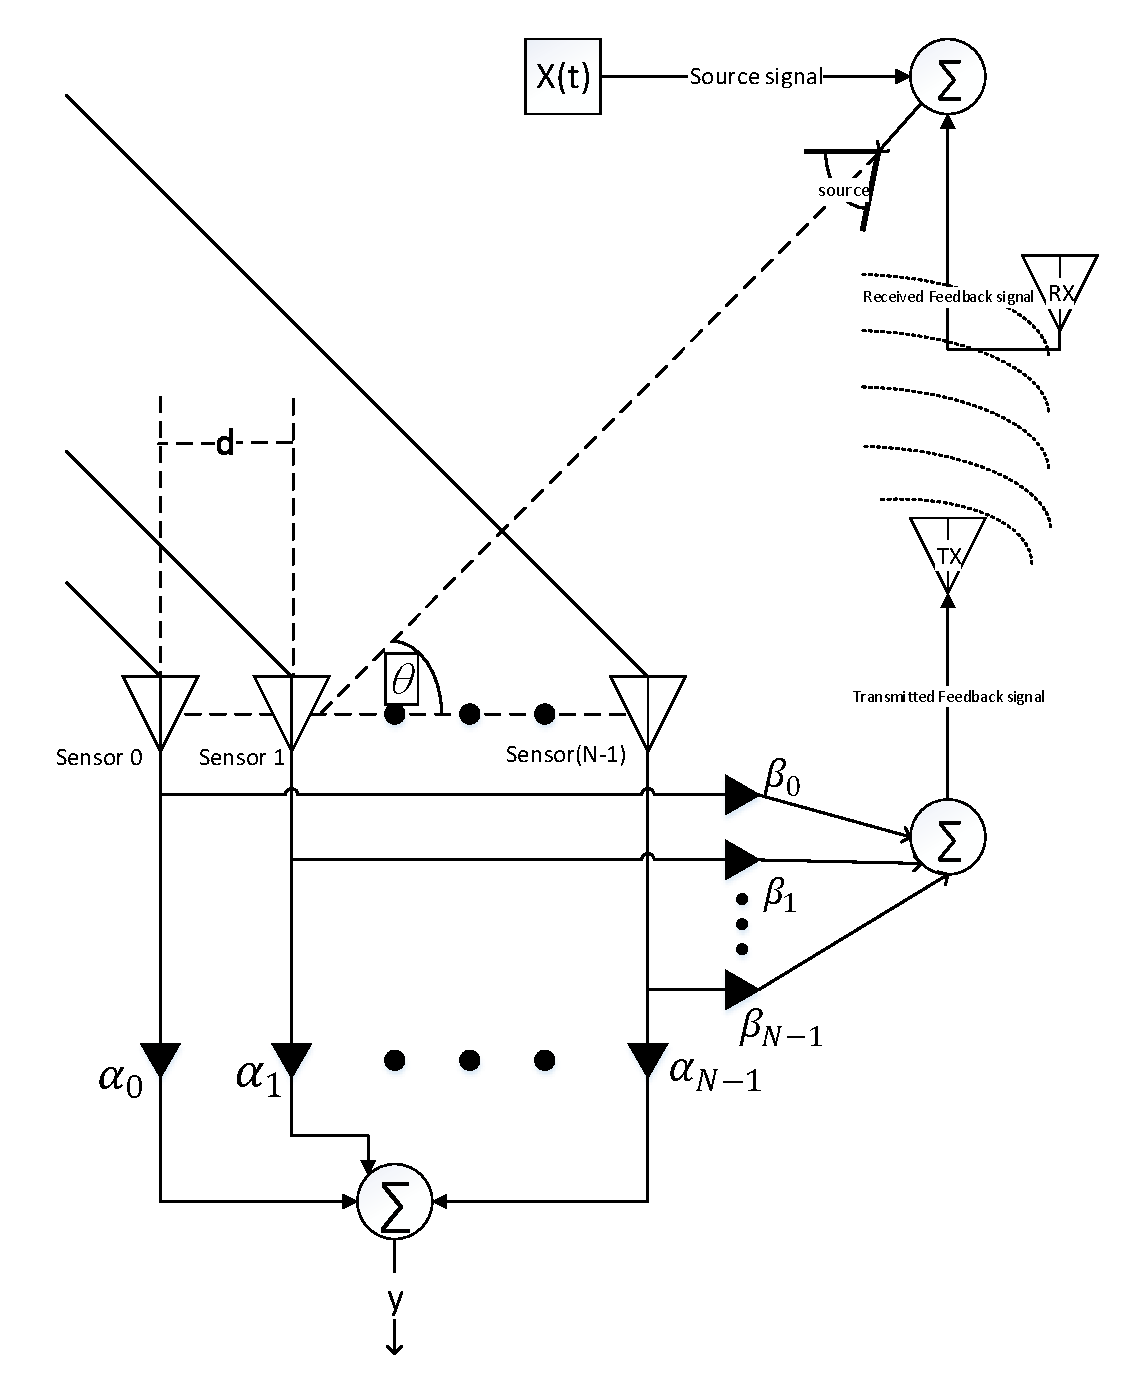
\includegraphics[width=0.7\textwidth]{./Media/SpatialIIR-diagram/SpatialIIR_VER4.pdf}
\caption
{
The proposed system: A far field source is received by an array. 
The received signal is also retransmitted back to the source. 
The latter has a transponder which feeds the signal back to the array.
}
\label{fig:SignalModel}
\end{center}
\end{figure}
By creating the suggested setup (fig.\ref{fig:SignalModel}), we aim to achieve a spatial-IIR which was previously discussed. 
By creating the suggested setup (fig.\ref{fig:SignalModel}), we aim to achieve a spatial-IIR which was previously discussed. 
Assume a far field source with signal $x(t)$. 
The resulting wavefront, with direction of arrival (DOA) $\theta$, is received by an array. 
For simplicity, we first assume a ULA, with elements spacing $d$. A weight and sum beamformer, with weights $\beta_n,\;n=0,...,N-1$  is used to retransmit the signal back to the source point. 
The retransmission can be conducted after RF modulation, or possibly acoustically, in the context of acoustical signal processing. 
As this cooperative source has a transponder, the obtained feedback signal, together with its own source signal $x(t)$ are summed up, and collected again by the array. 
A weight and sum beam-former, with weights $\alpha_n,\;n=0,...,N-1$ is used prior to generating the final output signal $y(t)$.
Possible implementation of this approach is a multiple-speaker spatial filtering (Fig. \ref{fig:SpatialIIR_StageApplication}), where the speakers are enhanced or filtered according to their location. 
The system may have a dynamic definition of its "hear-zones" which can be actively controlled by merely selecting the $ \vecnot{\alpha},\vecnot{\beta} $ coefficients.
\begin{figure}[!ht]
\begin{center}
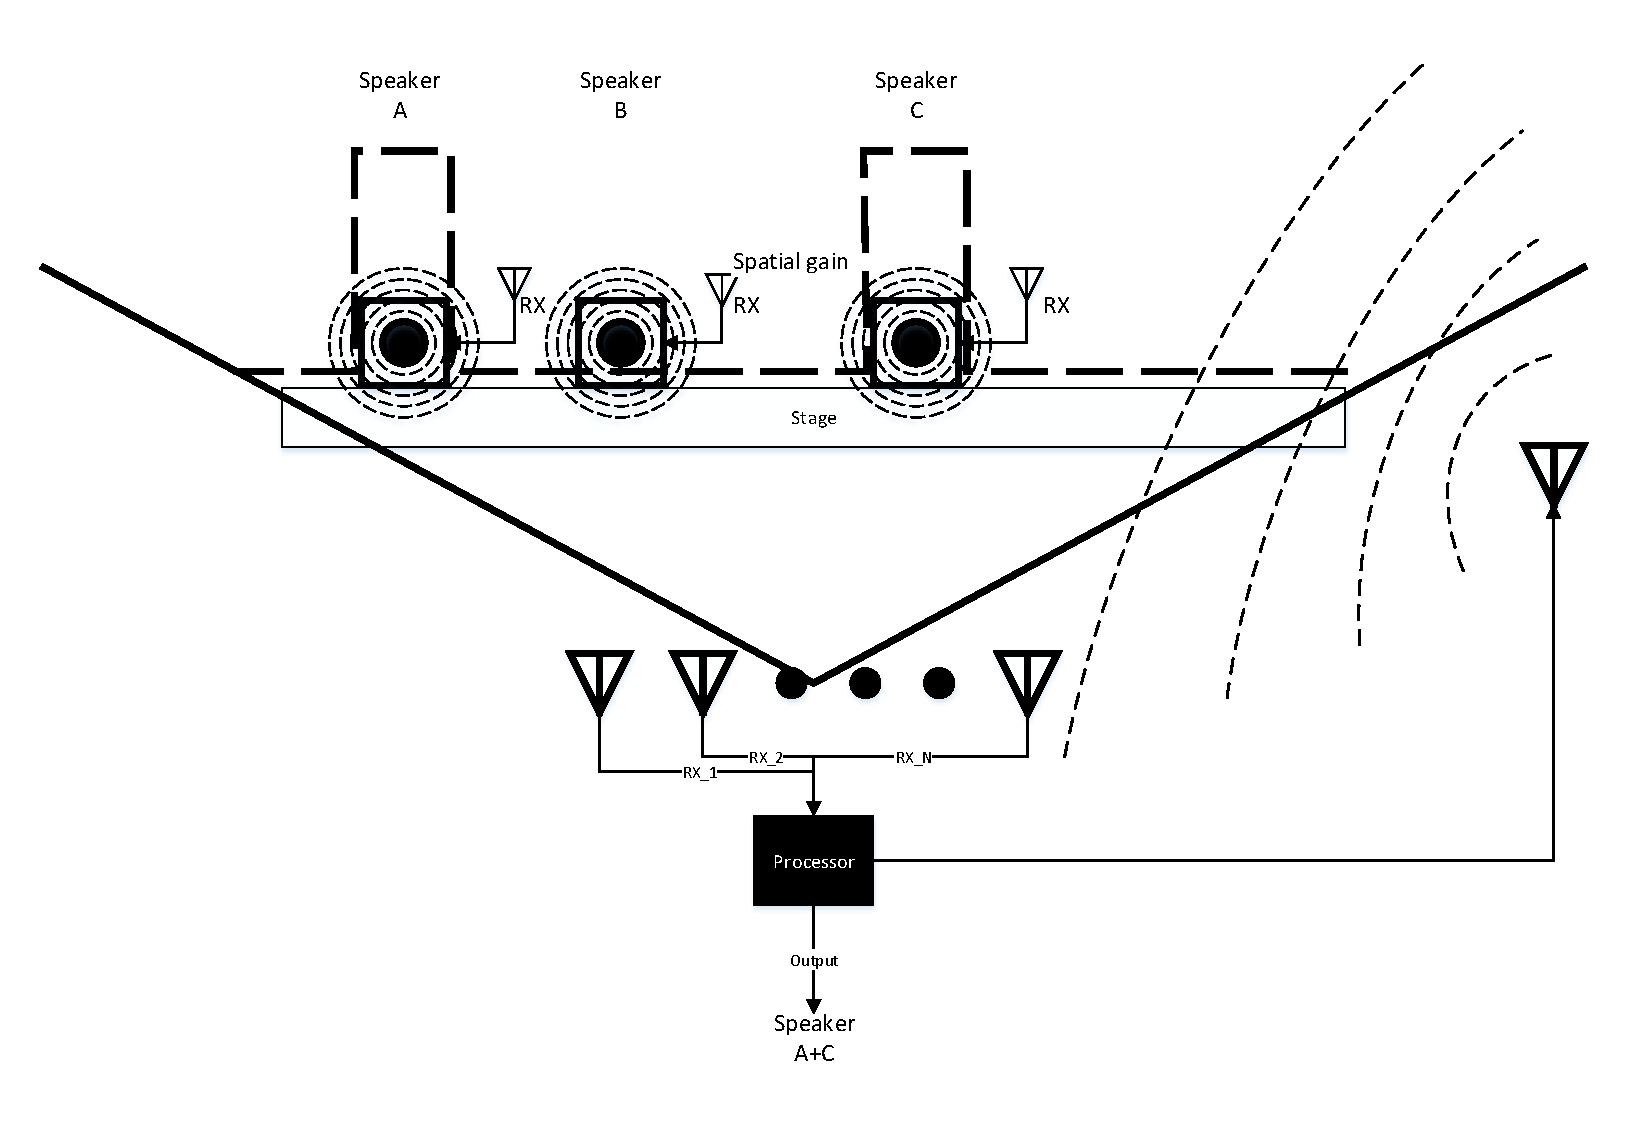
\includegraphics[width=0.7\textwidth]{./Media/SpatialIIR_Applications/SpatialII_StageApplication_VER3.pdf}
\caption
{
SpatialIIR - The multiple-speaker scenario. 
Speaker A and speaker C are in the pass-band of the spatial filter, while speaker B is supressed
}
\label{fig:SpatialIIR_StageApplication}
\end{center}
\end{figure}
Assuming a simple flat channel, the equation which defines the received signal at the n'th sensor, due to a wavefront from DOA $\theta$ is 
\begin{equation}
x_{n,\theta}(t) = x(t-\tau_{pd}-\tau_{n,\theta})+\sum_{m=0}^{N-1}{\beta_{m}x_{m,\theta}(t-\tau_{pd}-\tau_{tx}-\tau_{n,\theta})}
\label{eqn:SingleSensorTemporalEquality}
\end{equation}
where $ x(t) $ is the source signal, which travels in the medium with propagation speed of $ c $, $ x_{n,\theta}(t) $ is the $ n $'th sensor received signal due to wavefront from DOA $ \theta $, $ N $ is the number of sensors in the ULA, $ \tau_{pd}$ is the propagation delay from the source to the reference sensor, $ \tau_{tx} $ is the feedback transmission delay and $ \tau_{n,\theta}=n\frac{d\cos(\theta)}{c} $ is the sensor's location related delay (in case of ULA). 
It can be shown (see appendix \ref{apdx:MathDerv}) that with our approach one gets the transfer function of the overall system
$$
\ensuremath{
y_{\theta}^{\mathcal{F}}(\omega) 
=
\frac
{
\vecnot{\alpha}^{T}
\vecnot{d}_{\theta}
exp\left(-j\tau\right)
}
{
1
-
\vecnot{\beta}^{T}\vecnot{d}_{\theta}
exp\left(-j\tau\right)
}
x^{\mathcal{F}}(\omega)
}
$$
where $\vecnot{d}_{\theta}$ is the steering vector with n'th element $e^{-j\omega \tau_{n,\theta}}$ and $\vecnot{\alpha,\beta}$ are the coefficients vectors.
$^{T}$ stands for the transpose operator.
Some interesting observations rise from studying the system's transfer function.
\begin{itemize}
\item
{
The existence of a $ \theta $-dependent denominator weighted by coefficients $\vecnot{\beta}$ implies an actual IIR response in the spatial domain.
}
\item
{
For "non-cooperative" sources, there is no feedback channel (which is equivalent of setting $\vecnot{\beta} = 0 $), and we obtain the regular weight-and-sum beamformer with coefficients $\vecnot{\alpha}$.
}
\item 
{
The current form of the spatial filter requires knowledge of the forward and backward propagation delays $\tau_{pd},\tau_{tx}$.
}
\item 
{
The current form of the spatial filter assumes simplified one tap channels between the source and the array.
}
\end{itemize}
In this work we will investigate and develop methods of choosing the coefficients $ \vecnot{\alpha} $ and $ \vecnot{\beta} $ when a desired beam-pattern, $ H_{d}(\theta)$, is to be approximated. We will examine the outcome of partial knowledge of the propagation delays $\tau_{pd},\tau_{tx}$ and their influence on the stability of the filter. Another possible direction of research is to consider a more realistic reverberant channels which are common in acoustical environments, rather than the simple one-tap channel presented here. Simulations of dynamic spatial filtering of multi-speakers will be presented and compared to other conventional methods such as the classical delay and sum beam-former. Finally, we intend to implement the above suggested system.
\bibliographystyle{unsrt}
\bibliography{./Modules/Mendeley,./Modules/LocalBib}
\begin{appendices}
\chapter{Math derivations}
Time domain analysis of the proposed feedback based architecture, considering both propagation delay and attenuation, gives rise to
\begin{equation}
    \label{eqn:SingleSensorTemporalEquality}
    % \resizebox{.91\linewidth}{!}{
        \begin{split}
            x_{n}(t) = g\rBrace{s\rBrace{t-\tau_{pd}-\tau_{n}}
            +\sum_{m=0}^{N-1}{\alpha_{m}x_{m}\rBrace{t-\tau_{pd}-\tau_{n}}}},
        \end{split}
    % }
\end{equation}
where the first term of the right-hand side represents the contribution of the transmitted waveform $s(t)$ to the $n$'th array element and the second term represents the feedback contribution of the re-transmitted array signal to this same element.
Expressing \eqref{eqn:SingleSensorTemporalEquality}'s Fourier transform,
\begin{equation}
    \label{eqn_singleSensorFourier}
    % \resizebox{.91\linewidth}{!}{
        \begin{split}
            \F{x}_{n}\rBrace{\omega} =
            g\Bigg( & \F{s}\rBrace{\omega}
            \exp\rBrace{-j\omega\rBrace{\tau_{pd}+\tau_{n}}}
            \\&+\sum_{m=0}^{N-1}
            {
            \alpha_{m}\rBrace{\omega}\F{x}_{m}\rBrace{\omega}
            \exp\rBrace{-j\omega\rBrace{\tau_{pd}+\tau_{n}}}
            }\Bigg),
        \end{split}
    % }
\end{equation}
and its vector from,
$$
\F{\vx}\rBrace{\omega} = ge^{-j\omega\tau_{pd}} \rBrace{\F{s}\rBrace{\omega}+\vAlphaT \F{\vx}\rBrace{\omega}}\vd,
$$
we find that it can be simplified to
$$
\F{\vx}\rBrace{\omega} =\rBrace{I-g\vd\vAlphaT{}e^{-j\omega\tau_{pd}}}^{-1}g\vd\exp{\rBrace{-j\omega\tau_{pd}}}\F{s}\rBrace{\omega}.
$$
Then, denoting
\[
\phi\triangleq\omega\tau_{pd}
\]
as the round-trip signal propagation related electrical phase and using the Woodbury matrix identity \cite{woodbury1950inverting}, we find that
$$
\F{\vx}\rBrace{\omega}
=
\frac{    
g\vd\exp{\rBrace{-j\phi}}
}{
1 - g\aTd{}\exp{\rBrace{-j\phi}}
}\F{s}\rBrace{\omega}.
$$
Considering the noiseless case $\rBrace{\text{i.e. n}\rBrace{t}=0}$,
we express the general spatial response of FB as 
\begin{equation}
\label{eqn:GeneralFeedbackTransferFunction}
\Hba
\triangleq
\frac{\F{z}\rBrace{\omega}}{\F{s}\rBrace{\omega}} 
=
\frac{    
g\bTd{}\exp\rBrace{-j\phi}
}{
1 - g\aTd{}\exp\rBrace{-j\phi}
}.
\end{equation}
\par Note that this result confirms that our suggested array architecture achieves a controllable (via setting of $\vBeta$ and $\vAlpha$) and recursive (non-trivial denominator) spatial response.
As will be shown, high directivity and narrow beam-width are obtainable by proper selection of the weights. Comparing to traditional beamformers (i.e. with no feedback), the performance improvement will be expressed in terms of aperture increase, expressing the traditional beamformer aperture which achieves the same performance.
One may observe that opposed to traditional beamformers, the beampattern, $\Hba,$ is not only influenced by the impinging signal DOA, for it is also range selective due to its dependency on the phase parameter $\phi$.
As exemplified in Fig.~\ref{fig_rangeAzimuthSelectivity}, the combination of both angular and range selectivity enables the designer to enhance signals arriving from specific locations rather than only specific directions.
\begin{figure}[t!]
    \begin{center}
        \begin{overpic}[width=0.65\linewidth, 
        % grid, 
        tics=10,trim=0 0 0 0]{./Media/azimuthRangSelectivity.png}
            \put (20, 23){\rotatebox{0}{\footnotesize{Angular response}}}
            \put (30.5, 47){\rotatebox{0}{\footnotesize{Enhanced radial slice}}}
        \end{overpic}
    \end{center}
     \caption{A visualization of the spatial area selectivity concept. Combining both radial selectivity (i.e. enhancing signals from a specific distance) and DOA-based selectivity, allows the enhancement of signals arriving from specific areas (grey filled), while signals originated in other areas (even from the same DOA) are suppressed.}
    \label{fig_rangeAzimuthSelectivity}
\end{figure}
\label{apdx:MathDerv}
\end{appendices}
\end{document}